\subsection{Interpretacion de los datos. Vocabulario y terminologia}

Recordemos que el objetivo principal del acceso a los datos, es obtener conocimiento. Hay que tener en 
cuenta que los datos por si solos, no tienen ningun valor, ya que carecen de sentido, una vez integrados en un contexto,
nos aportara informacion, y procesando y analizando esta informacion, se obtendra el conocimiento.\\
    
\begin{figure}[ht]
    \centering 
    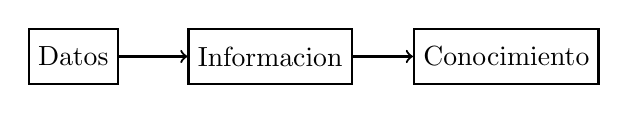
\begin{tikzpicture}[thick]
        \node[draw,rectangle,minimum size=20] (a) {Datos};
         \node[draw,rectangle,minimum size=20,right of= a, node distance=2.5cm] (b) {Informacion};
         \node[draw,rectangle,minimum size=20,right of=b, node distance=3cm] (c) {Conocimiento};
         \draw[->] (a) to (b);
        \draw[->] (b) to (c);
     
      \end{tikzpicture}
      \caption{Diagrama. De datos a conocimiento}
    \end{figure}
 
Para poder obtener este conocimiento de los datos, es necesario que el usuario interprete correctamente los datos, por lo
que el usuario debe contar con conocimientos en la materia o realizar una tarea de investigacion, que le permita 
entender los datos extraidos. 

Asi pues, para que el usuario pueda obtener la informacion de una manera directa, requiere de conocimientos tanto 
de programacion como especificos de la materia y los recursos para crear una infraestructura que le permita implementar 
una representacion de los datos que le sea util.

Podemos concluir que el acceso a los datos por parte del usuario medio, no es directa.\\

Para poder construir un sistema que haga los datos accesibles, es imprescindible disenar un modelo  para concretar la 
informacion que se desea obtener. El diseno de un sistema permitira que a partir de unos valores dados, proporcione unos resultados.
Para ello sera necesario tener un conocimiento solido del conjunto de datos que se necesita, los valores,
sus unidades y como se relacionan entre si.


\subsubsection{How to solve it} 
Estudiar el objetivo buscado y recurrar a la ayuda de expertos si fuera necesario para adquirir los conocimientos necesarios
sobre la materia. Disenar un modelo que proporcione la informacion que buscamos. Este modelo debera proporcional la informacion 
al usario en un lenguaje o formato compresible. Si no es posible proporcionarmos las herramientas necesarias para que este pueda 
comprender el contexto de la informacion.

\subsubsection{How we solve it. Aire Guru} 
Aire Guru se ocupa de representar el EAQI (European Air Quality Index) general calculado sobre un mapa. Este es un formato mas legible para los usuarios.
Este indice mustra un indicador con cinco niveles: "Insalubre" "Malo" "Pobre" "Aceptable" y "Bueno" y especifica un rango de colores desde el rojo hasta el celeste.\\
\newpage
\begin{figure}[ht]
    \centering
    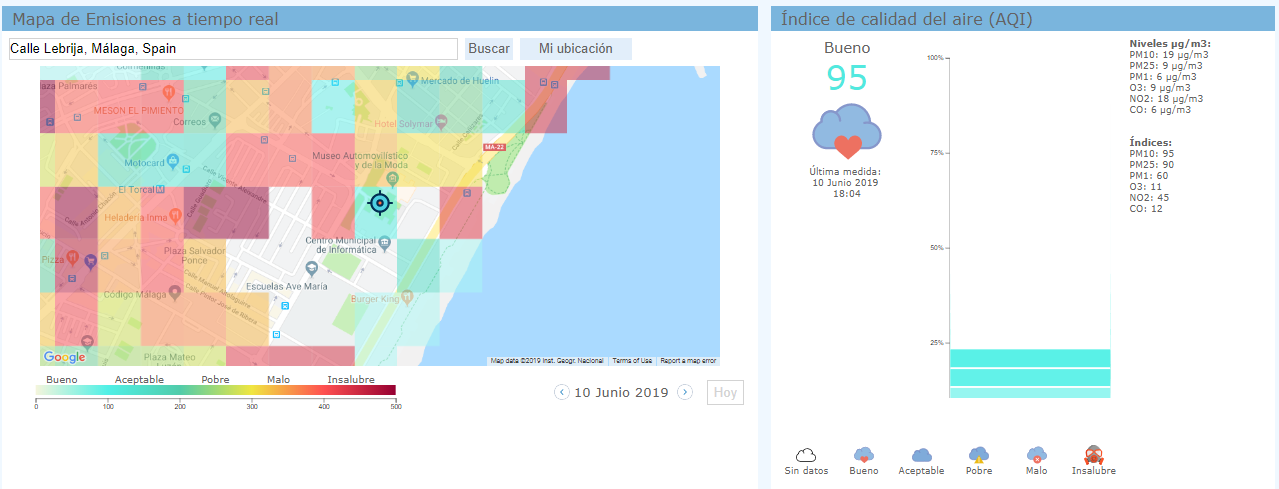
\includegraphics[width=10cm]{mapAireGuru}
    \caption{Aire Guru. Landing page. Top section}
\end{figure}

Nuestra plataforma introduce ademas una iconografica para ayudar al usuario a tener una idea directa de la situacion, ya que son mas 
explicativos que los colores. En caso de peligro, queda bien representado con el color rojo, pero en el caso del azul o verde, en nuestra cultura, no
tenemos definido un estado para estos colores.\\
\begin{figure}[ht]
    \centering
    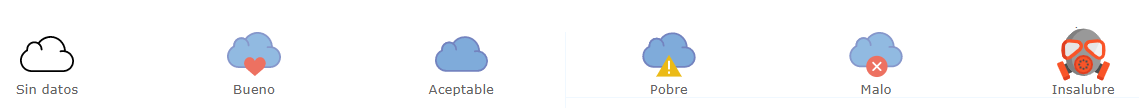
\includegraphics[width=12cm]{EAQUI_Icons}
    \caption{Iconografica Aire Guru}
\end{figure}

Ademas proporciona un glosario con las descripciones de los agentes contaminantes, complicaciones medicas, fuentes de contaminacion
y la iconografia utilizada y una ayuda donde se puede consultar el calculo de AQI y ampliar informacion.

La herramienta Aire guru presenta la informacion en el idioma nativo de la ciudad y se utiliza un lenguaje sencillo y directo.
Ademas se utiliza el mismo estilo, colores e iconografia en todo el diseno para que el usuario se familierize rapidamente y pueda
prestar atencion al significado de los datos en vez de perderse en el diseno e intentar encontrar su significado.

Aire Guru se comprende de distintas secciones disponibles para todos los usuarios. En la zona superior, podemos ver el mapa que mediante la seleccion de un punto, nos
mostrara informacion detallada de este punto. A continuacion, cuenta con una seccion que filtrara la informacion acorde a las preferencias del usuario
y para concluir, muestra el historial de los contaminantes desde 2018.
Ademas, para usuarios identificados, mostrara directamente la informacion de su localizacion y mostrara al usuario su historial personal
con la polucion a la que ha estado rodeado.

El workflow de las distintas secciones de Aire Guru esta detalladamente estudiada. Como vemos en la Figura X. Aire Guru. Landing page. Top section, el punto de partida es la localizacion que nos interesa,
a continuacion se muestra la informacion general de este punto, el AQI general, despues el AQI de cada uno de los contaminantes que componen el 
AQI general y por ultimo los valores numericos de cada uno de los contaminantes. Como vemos vamos de menos a mas detalle.

\paragraph{Evaluation} \mbox{} 

\begin{itemize}
\done El lenguaje utilizado en toda la herramienta es un lenguaje comun, huye de la terminologia cientifica pero proporciona la informacion
suficiente para enteder la situacion.
\crossed Algunos terminos especificos no se han podido sustituir como "Indice de calidad del Aire".
\done Se han proporcionado la herramientas necesarias para entender el concepto. Se ha utilizado la norma europea de calidad del aire para 
representar los valores y se ofrece al usuario recursos en la pagina para su comprension ademas de recursos extenos.
\end{itemize}

\newpage